\documentclass[12pt,a4paper,twoside]{article}
\usepackage{url}
\usepackage{hyperref}
\usepackage[francais]{babel}
\usepackage{fancyhdr}
\usepackage{lastpage}
\usepackage{a4wide} 
\usepackage{amsmath}
\usepackage{amssymb} 
\usepackage{graphicx}
\usepackage{color}
\usepackage{fancybox}
\usepackage{moreverb}
\usepackage[T1]{fontenc}
% \usepackage{hangcaption}
\usepackage{listings}
\usepackage{setspace}
\usepackage[utf8x]{inputenc}


\title{Introduction à la Recherche en Laboratoire}
\author{Gaétan Bahl}
\date{\today}

\pagestyle{headings}

\begin{document}
\pagenumbering{roman}
\lstset{ numbers=left, tabsize=3, frame=single, numberstyle=\ttfamily, basicstyle=\footnotesize} 
\thispagestyle{empty}

\begin{center}
\makebox[\textwidth][l]{
\raisebox{-8pt}[0pt][0pt]{

\includegraphics[height=2cm]{Images/logo_ljk.png}
}
}
\makebox[\textwidth][r]{
\raisebox{0pt}[0pt][0pt]{

\includegraphics[height=2cm]{Images/logo_ensimag}
}
}
Grenoble INP  -- ENSIMAG\\
Ecole Nationale Supérieure d'Informatique et de Mathématiques Appliquées\\
\vspace{3cm}
{\LARGE Introduction à la Recherche en Laboratoire}\\
\vspace{1cm}
Effectuée au Laboratoire Jean Kuntzmann dans l'équipe EDP\\
\vspace{2cm}
\shadowbox{
\begin{minipage}{1\textwidth}
\begin{center}
{\Huge Solutions de viscosité d'équations aux dérivées partielles et schémas numériques associés }\\
\end{center}
\end{minipage}
}\\
\vspace{2cm}
Gaétan Bahl\\
Élève en 2A MMIS\\
\vspace{3mm}
2015-2016\\
\vspace{2,5cm}
\begin{tabular}{p{10cm}p{10cm}}
{\bf Laboratoire Jean Kuntzmann}                                            &{\bf Encadrant}\\
{\footnotesize 51, rue des Mathématiques}     & Emmanuel Maître\\
{\footnotesize BP 53}      	& {\footnotesize Équipe EDP }\\
  {\footnotesize 38041 Grenoble Cedex 9}			& \\
{} 		 & {} \\		
\end{tabular}
\end{center}

\newpage

\begin{center}

	{\huge Résumé} \\ 
\end{center}
	\vspace{2cm}

	Ce document présente les travaux que j'ai effectués dans le cadre du module d'Introduction à la Recherche en Laboratoire, au cours du second semestre de ma deuxième année à l'Ensimag, en filière Modélisation Mathématique, Image, et Simulation.

	Ces travaux on été réalisés au Laboratoire Jean Kuntzmann (LJK-IMAG), au sein de l'équipe Équations aux Dérivées Partielles (EDP) et sous la tutelle d'Emmanuel Maître, 
professeur à Grenoble INP et membre de cette équipe.

	Les connaissances utilisées pour ces travaux ne s'inscrivent pas intégralement dans le cursus de l'Ensimag, la notion de solution de viscosité n'y étant pas étudiée.
Les cours de MMIS permettent néanmoins de mieux les aborder, en particulier le module \emph{Modèles EDP et Schémas Numériques en Sciences de l'Ingénieur}, enseigné par Emmanuel Maître au premier semestre de deuxième année. \\

	Cette Introduction à la Recherche en Laboratoire s'intéresse à une nouvelle notion de solution d'équations aux dérivées partielles, plus générale que les définitions classiques. 
Ceci permet de considérer des cas que les définitions classiques ne permettent pas de résoudre. Nous nous sommes plus spécifiquement intéressés à ce que cette nouvelle notion 
peut nous apporter dans le cadre du transport optimal, en implémentant et optimisant un schéma numérique résolvant l'équation de Monge-Ampère.


\newpage

\begin{center}

	{\huge Remerciements} \\ 
\end{center}
	\vspace{2cm}
    Je tiens à remercier Emmanuel Maître, non seulement pour m'avoir permis de réaliser cette Introduction à la Recherche en Laboratoire, mais aussi pour sa patience, sa pédagogie, et son aide précieuse. \\
    

    Je tiens également à remercier l'équipe EDP du laboratoire Jean Kuntzmann, pour son accueil chaleureux et pour m'avoir permis d'assister à leurs nombreux et très intéressants séminaires, qui m'ont permis de découvrir des applications des équations aux dérivées partielles et de mieux comprendre leurs enjeux dans le monde contemporain. \\
    



\newpage

\tableofcontents

\newpage
\pagenumbering{arabic}
\setcounter{page}{1}
%\begin{spacing}{2.5}


\section{Introduction}

La notion de solution de viscosité a été introduite au début des années 80 par Pierre-Louis Lions et Michael G. Crandall \cite{crandall1983viscosity}. 
Il s'agit d'une généralisation de la notion de solution d'Équation aux Dérivées Partielles. 
Cette notion peut être utile dans la résolution d'EDP linéaires, telles que l'équation de la chaleur, mais elle est surtout utile dans le cadre d'équations non-linéaires. 
Elle n'est en général \emph{pas} utilisée dans la résolution de systèmes d'équations (ex. Navier-Stokes) \cite{dragoniintroduction}.

Le but de cette IRL a tout d'abord été de comprendre la notion de solution de viscosité, puis d'implémenter sous
Scilab un schéma numérique convergeant vers une solution de viscosité de l'équation de Monge-Ampère pour le transport optimal, et enfin de
ré-implémenter ce schéma sous OpenCL, afin de l'exécuter rapidement sur un processeur graphique.

\section{Solutions de Viscosité}

\subsection{Rappels sur les Équations aux Dérivées Partielles}

Commençons par rappeler quelques définitions, afin de mieux situer le contexte du sujet.

\paragraph*{Définition : Equation aux Dérivées Partielles } 

Une Équation aux Dérivées Partielles (EDP) d'ordre $k$ est une équation liant une fonction inconnue u
et ses dérivées jusqu'à l'ordre $k$. \\

En particulier, nous nous intéresserons au cas $k=1,2$, c'est-à-dire :

\begin{align}  
k=1, & \; F(x,u,Du) = 0, x\in \Omega \subset \mathbb{R}^n, \label{eq:edp}\\
k=2, & \;  F(x,u,Du,D^2u) = 0, x\in \Omega \subset \mathbb{R}^n, \label{eq:edp2}
\end{align}

où $F : \Omega \times \mathbb{R} \times \mathbb{R}^n \times \mathcal{M}_{n,n} \to \mathbb{R}$.

\paragraph*{Définition : EDP linéaire}

Une Équation aux Dérivées Partielles est dite \emph{linéaire} si elle peut s'écrire sous la forme :

$$ Lu = f(x) $$

où $L$ est un opérateur différentiel linéaire d'ordre $k$. Dans tous les autres cas, l'EDP est dite \emph{non-linéaire}.

L'équation de la chaleur, par exemple, est linéaire :

\begin{equation}
\frac{\partial u}{\partial t} - \Delta u = 0
\end{equation}


\paragraph*{Solution classique d'une EDP}

Une fonction $u : \Omega \to \mathbb{R}^n$ est appelée \emph{solution classique} de l'EDP \ref{eq:edp} d'ordre $k$ si elle est $\mathcal{C}^k$ et satisfait l'EDP $\forall x \in \Omega$.


\subsection{Justification de la nécessité des solutions de viscosité}


Considérons l'équation eikonale (avec $f \equiv 1$) dans le problème de Dirichlet suivant :

\begin{equation} \label{eq:eikonal}
    \begin{cases}
        |Du| = 1, \; x \in [-1, 1] \\
        u(x) = 0, \;  |x| = 1
    \end{cases}
\end{equation}

Supposons qu'il exite $u$ solution classique de \ref{eq:eikonal}. $u$ est alors $\mathcal{C}^1$.
On a $u(-1) = u(1) = 0$. Par le théorème des accroissements finis, il existe alors $x_0 \in ]-1,1[$ tel que  
$u'(x) = 0$. Puisque $u$ est $\mathcal{C}^1$ il existe alors un voisinage de $x_0$ où $|u'(x)| < 1$. 
$u$ ne peut donc pas être solution de \ref{eq:eikonal}. C'est pourquoi nous avons besoin d'une notion de solution
plus faible.

\subsection{Définition d'une solution de viscosité}

La définition d'une solution de viscosité et des explications plus détaillées  peuvent  être trouvées dans 
\cite{bressan2010viscosity}. Nous en donnerons ici une explication intuitive dans un exemple en une dimension. 

Afin de définir la notion de solution de viscosité, nous avons tout d'abord besoin de parler de \emph{sous-différentielle} et de \emph{sur-différentielle}.

\paragraph*{Définition : Sous-différentielle}

Soit $u : \Omega \to \mathbb{R}$. Un vecteur $p$ est un sous-gradient (resp. sur-gradient) de $u$ en un point $x$ si la droite orientée par $p$ est tangente sous (resp. sur) la courbe de $u$ en $x$. La figure ~\ref{sousgradient}
montre un exemple de deux sous-gradients.

\begin{figure}
\begin{center}
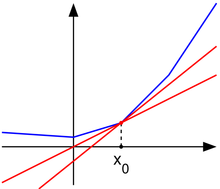
\includegraphics[scale=0.7]{Images/sousgradient.png}
\caption{Sous-gradient (tiré de Wikipedia.fr)}
\label{sousgradient}
\end{center}
\end{figure}

On note l'ensemble des sous-gradients (resp. sur-gradients) de $u$ en $x$ : $D^{+}u(x)$ (resp. $D^{-}u(x)$). \\


\paragraph*{Définition alternative : Sous-différentielle}

Une définition alternative très utile  de la notion de sous-différentielle d'une fonction $\mathcal{C}^k$ est la suivante : \\

On a $p \in D^{+}u(x)$ (resp. $D^{-}u(x)$) si et seulement si il existe une fonction $\phi \in \mathcal{C}^1 (\Omega)$
telle que $\nabla \phi(x) = p$ et $u - \phi$ admet un minimum (resp. maximum) local en $x$.

Intuitivement, c'est le fait qu'il existe une fonction régulière dont la courbe touche celle de $u$ en $x$
et dont la dérivée est $p$. Un exemple est donné par la figure ~\ref{sousdiff}.

\begin{figure}
\begin{center}
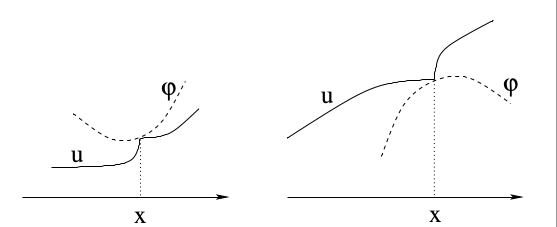
\includegraphics[scale=0.6]{Images/sousdiff.png}
\caption{Sous-différentielle (tiré de \cite{bressan2010viscosity})}
\label{sousdiff}
\end{center}
\end{figure}

Ces définitions s'appliquent également aux dérivées d'ordres supérieurs.


\paragraph*{Définition : Solution de viscosité}

Une fonction $u$ est une \emph{sous-solution de viscosité} de \ref{eq:edp} si 

$$F(x,u(x),p) \leq 0, \forall x \in \Omega, p \in D^{+}u(x) $$

Une fonction $u$ est une \emph{sur-solution de viscosité} de \ref{eq:edp} si 

$$F(x,u(x),p) \geq 0, \forall x \in \Omega, p \in D^{-}u(x) $$

Une fonction $u$ est une \emph{solution de viscosité} si elle est à la fois une \emph{sur-solution} et une 
\emph{sous-solution} de viscosité.


\subsection{Applications possibles des solutions de viscosité}

Voici quelques exemples d'EDP non-linéaires pour lesquels les solutions de viscosité sont utiles \cite{dragoniintroduction}. Le contrôle optimal est une des applications principales des solutions de viscosité, en finance notamment. Une liste très fournie d'applications peut être trouvée dans \cite{crandall1992user}.

\paragraph*{Équation de Hamilton-Jacobi}

$$ H(x,u,Du) = 0$$

où $H$ est le \emph{Hamiltonien}.

Cette équation est très importante en contrôle optimal et en économie, en particulier quand elle prend la forme 
\emph{Hamilton-Jacobi-Bellman} \cite{bardi2008optimal}.

\paragraph*{Mean Curvature Motion}

$$\displaystyle u_t - \Delta u + \langle D^2 u \frac{Du}{|Du|}, \frac{Du}{|Du|} \rangle  $$

Cette équation de géométrie différentielle décrit l'évolution d'une hypersurface essayant de minimiser son aire, elle
a des applications en physique.


\paragraph*{Equation de Monge-Ampère}

$$ \det(D^2 u) = f(x) $$

Cette équation a des applications en transport optimal, et c'est sur celle-ci que nous avons choisi de nous concentrer.

\section{Solutions de viscosité : Exemples }

Nous allons maintenant voir quelques exemples de solutions de viscosité.

\subsection{Exemple 1D : Équation eikonale}

Nous revisitons ici l'équation eikonale 
\begin{equation} \label{eq:ek}
 - |Du| + 1 = 0, 
\end{equation}
que nous avons vue plus haut. 

Il s'agit de montrer que $u(x) = 1 - |x|$ en est solution de viscosité sur $ [-1;1]$.


\begin{figure}
\begin{center}
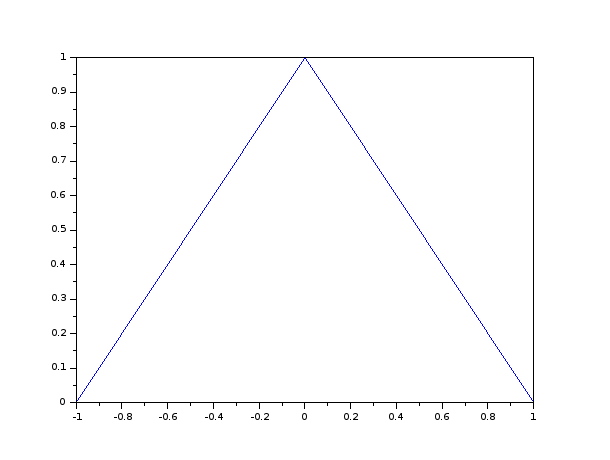
\includegraphics[scale=0.5]{Images/eikonale.png}
\caption{Solution de viscosité de l'équation eikonale}
\label{eikonale}
\end{center}
\end{figure}

Sur $[-1,0[$ et $]0,1]$, $u$ est différentiable et vérifie l'équation eikonale. La condition de
sur-solution et de sous-solution est donc vérifiée sur ces intervalles.

Le problème se situe en
0, où $u$ n'est pas différentiable.

On a clairement $D^{+}u(0) = [-1; 1]$. 
On a donc bien $\forall p \in D^{+}u(0), \; - |p| + 1 \geq 0$, donc $u$ est une sous-solution de viscosité
de l'équation \ref{eq:ek}.

On voit également que $D^{-}u(x) = \emptyset$, la propriété de sur-solution est donc trivialement vérifiée en 0. \\

$u$ est donc bien une solution de viscosité de \ref{eq:ek}.



\subsection{Exemple 2D : Monge-Ampère}

Le but est ici de prouver numériquement que $u(x) = \frac{1}{2}((|x|-1)^{+})^2$ est bien solution de viscosité de l'équation de Monge-Ampère : $\det(D^2 u(x) )= f(x)$, quand $f(x) = (1 - \frac{1}{|x|})^{+}$.

\begin{figure}[!h]
\begin{center}
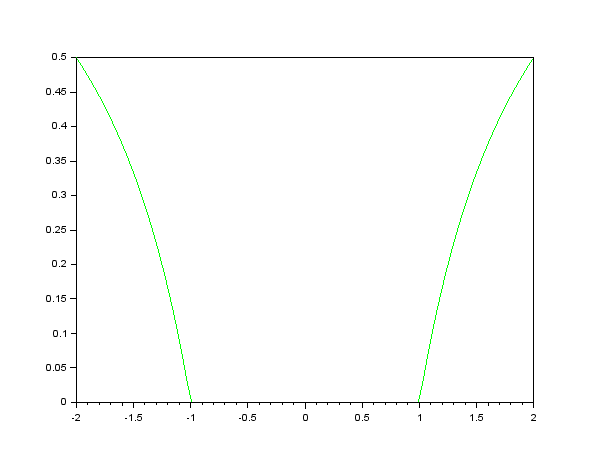
\includegraphics[scale=0.5]{Images/fig4.png}
\caption{fonction f} 
\end{center}
\end{figure}

\subsubsection{Étude de la fonction u}


On commence par représenter la fonction u sur $[-2,2]\times[-2,2]$ (figure \ref{fonctionu}).

\begin{figure}[!h]
\begin{center}
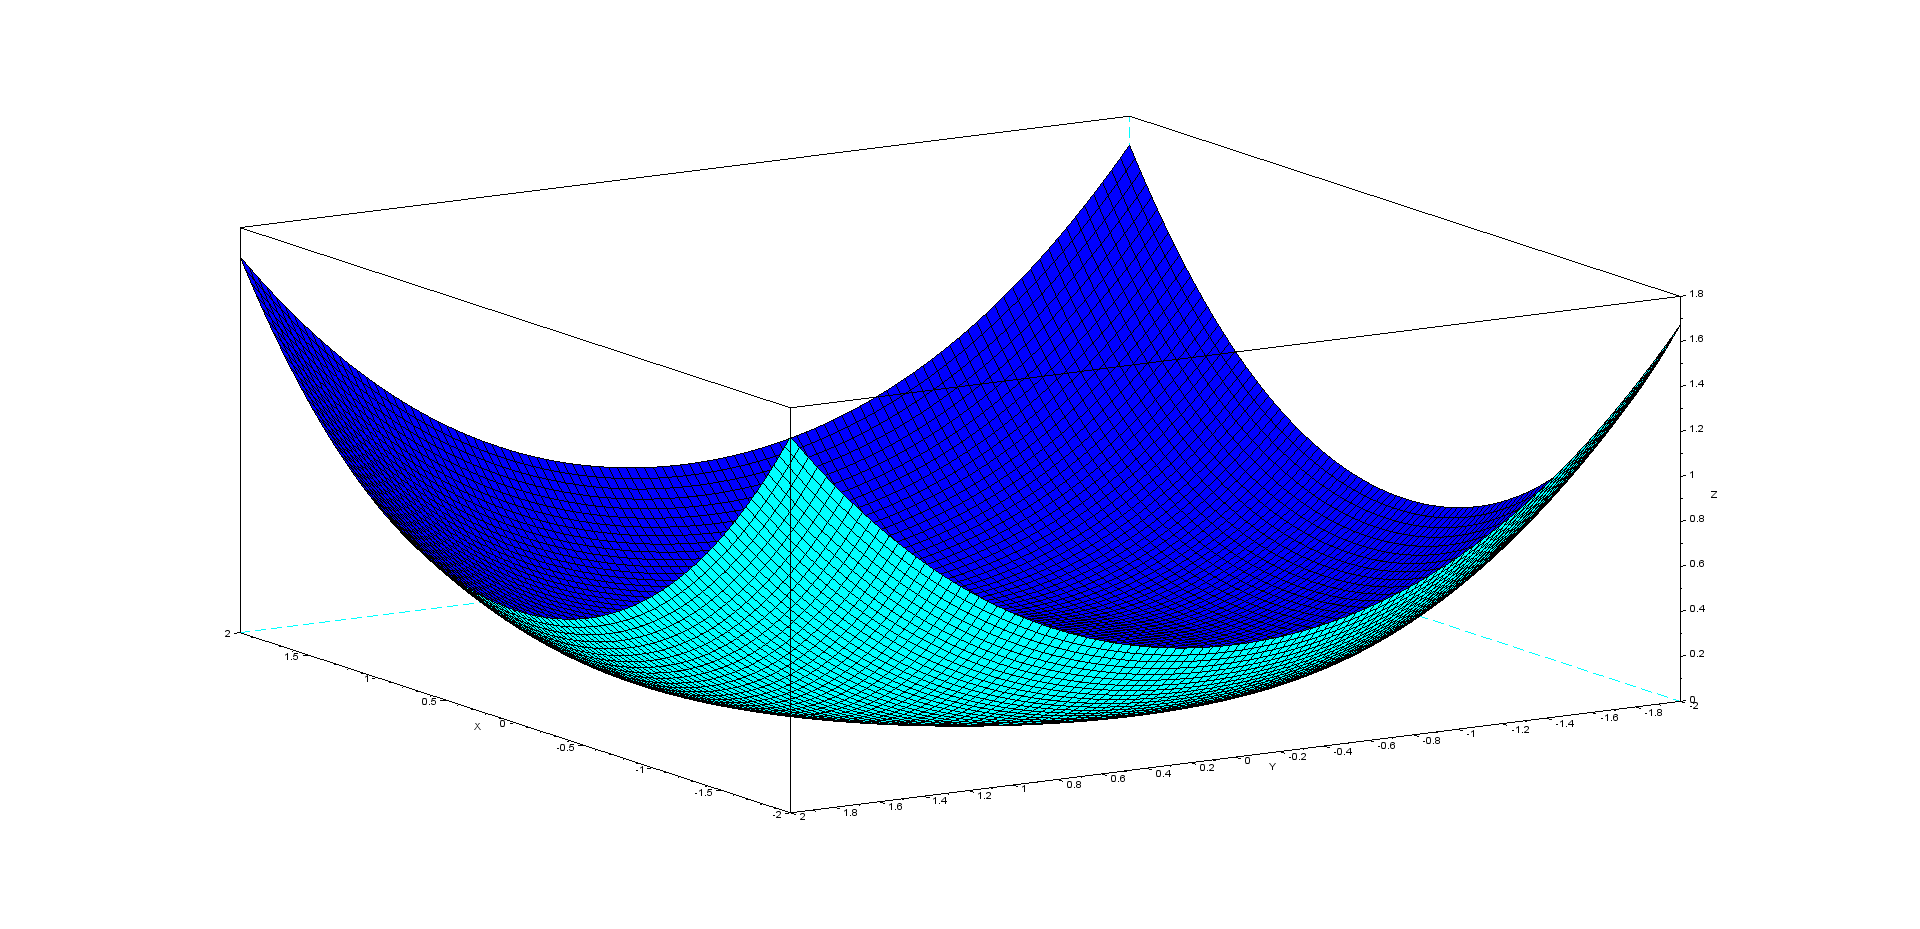
\includegraphics[scale=0.25]{Images/fig1.png}
\caption{fonction u vue d'au dessus}
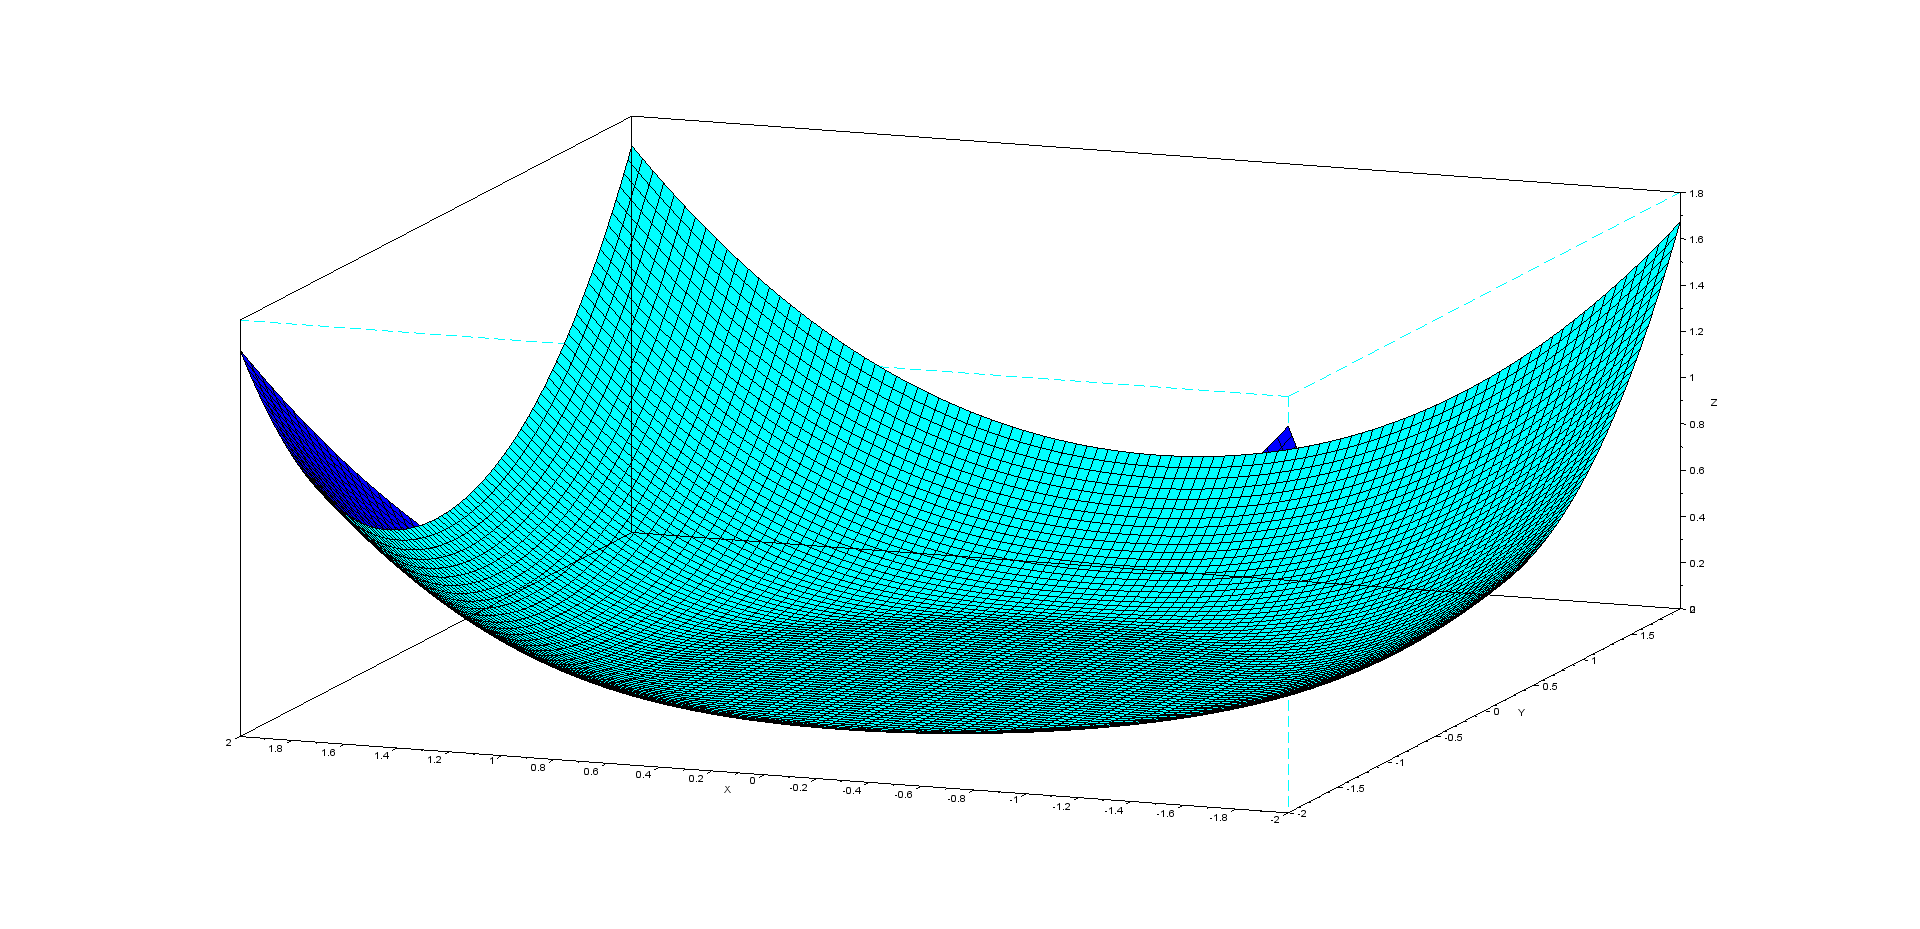
\includegraphics[scale=0.25]{Images/fig0.png}
\caption{fonction u vue d'en-dessous}
\label{fonctionu}
\end{center}
\end{figure}

On obtient une cuvette avec un fond plat. Cela se voit mieux lorsqu'on réalise une coupe de la courbe (figure \ref{coupeu}).


\begin{figure}[!h]
\begin{center}
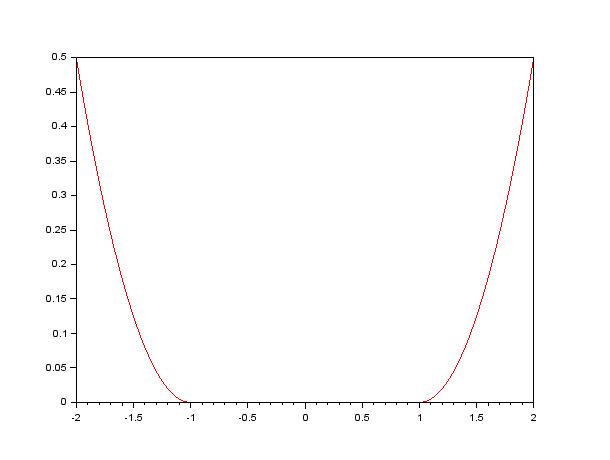
\includegraphics[scale=0.5]{Images/fig3.png}
\caption{fonction u dans le plan y = 0}
\label{coupeu}
\end{center}
\end{figure}

La fonction est $C^2$ partout, sauf sur le cercle unité.

\subsubsection{Vérification de l'équation}

Pour montrer que $u$ vérifie l'équation de Monge-Ampère, on calcule le déterminant de sa Hessienne, et on le compare à $f$. Puisqu'on peut construire $u$ par révolution autour de l'axe des $z$, on se cantonne au plan $y=0$.

On obtient la figure \ref{hessienne}.


\begin{figure}[!h]
\begin{center}
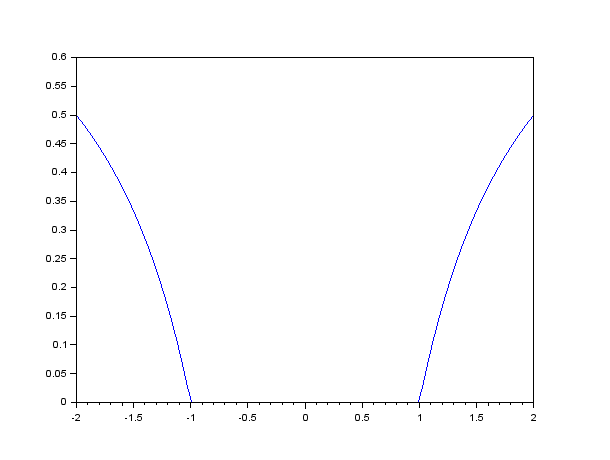
\includegraphics[scale=0.5]{Images/approxhessian.png}
\caption{$\det(D^2 u)$ : membre de gauche de l'équation de Monge-Ampère}
\label{hessienne}
\end{center}
\end{figure}

En soustrayant f à ce résultat, on obtient le résultat de la figure \ref{difff}.

\begin{figure}[!h]
\begin{center}
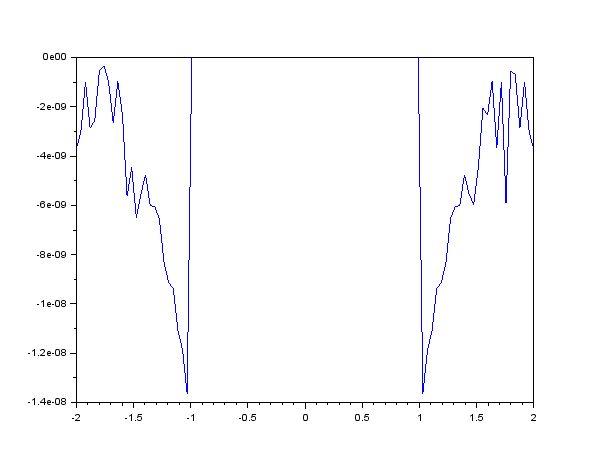
\includegraphics[scale=0.5]{Images/erreur.png}
\caption{Différence entre le membre de gauche et le membre de droite}
\label{difff}
\end{center}
\end{figure}


On voit que le résultat est très proche de $f$, à part sur le cercle unité, ce qui était attendu.

\subsubsection{$u$ est $C^1$}

On étudie maintenant la fonction $u$ en $(1,0)$. On sait que $u(1,0)=0$ et on veut étudier numériquement sa régularité en ce point.

On utilise le code Scilab suivant pour approximer $u'(1^{+},0)$ par $\frac{u(1 + dx)}{dx}$ en faisant tendre $dx > 0$ vers $0$ :

\begin{lstlisting}[frame=single, language=Scilab]
for i = 1:10
    dh = 10^(-i);
    disp(u(1+dh, 0)/dh);
end
\end{lstlisting}

Et on obtient : 

\begin{lstlisting}[frame=single, language=Scilab]
    0.05  
    0.005  
    0.0005  
    0.00005  
    0.000005  
    0.0000005  
    5.000D-08  
    5.000D-09  
    5.000D-10  
    5.000D-11  
\end{lstlisting}

De plus, $u'(x,0)=0$ pour $x \in [-1,1]$, on a donc vérifié numériquement que $u$ est $C^1$.

\subsubsection{Calcul des sous-gradients de $u$ en $(1,0)$}

Comme pour $u'$, on approxime $u''(1^{+},0)$ par $\frac{u(1+2dx,0) -2u(1+dx,0)}{dx^2}$, et on fait tendre $dx > 0$ vers $0$.

On obtient :


\begin{lstlisting}[frame=single, language=Scilab]
    1.  
    1.  
    1.  
    1.  
    1.  
    1.  
    1.  
    1.  
    0.9999997  
    1.0000002  
\end{lstlisting}

Ce qui nous donne que $D^{-}u'(1,0)=[0,1] $, car à gauche, $u''(1^{-},0)=0$.


\section{Résolution numérique de l'équation de Monge-Ampère}

\subsection{Présentation}

La suite du sujet consistait en l'implémentation d'une méthode de résolution numérique. Nous avons choisi de 
travailler sur l'équation de Monge-Ampère, appliquée au transport optimal, en implémentant une méthode 
proposée dans \cite{benamou2014numerical}.


Le transport optimal est un problème connu ayant beaucoup d'applications, mais dont les méthodes de résolution
restent sous-développées par rapport à la théorie qui, elle, est bien établie \cite{villani2008optimal}. \\


Le problème est le suivant : \\

Nous disposons de deux mesures de probabilité, $\rho_X$ sur $X$ et $\rho_Y$ sur $Y$,
avec $X,Y \in \mathbb{R}^n$. Il s'agit de trouver une application $\mathbb{M}$ appartenant à l'ensemble des applications 
transformant la densité $\rho_Y$ en la densité $\rho_X$,
$\lbrace T : X \to Y, \rho_Y(T) \det(\nabla T) = \rho_X \rbrace$.

Cette application doit être optimale au sens de la fonction de coût quadratique :

$$\frac{1}{2} \int_X ||x-T(x)||^2\rho_X(x) dx $$

Cela nous donne donc l'équation de Monge-Ampère suivante : 

\begin{equation}
\det(D^2 u) = \frac{\rho_X}{\rho_Y(\nabla u)}, \; x \in \Omega
\end{equation}


Dans \cite{benamou2014numerical}, la condition au bord est donnée par une équation de Hamilton-Jacobi, le but
étant d'envoyer le bord de $X$ sur le bord de $Y$ :

\begin{equation}
H(\nabla u(x)) = dist(\nabla u(x), \partial Y) = 0, \; x \in \partial \Omega
\end{equation}

\subsection{Exemple analytique}

Commençons par un exemple analytique de mappage d'une densité sur une autre à l'aide d'une application que l'on choisit
à la main. De cette manière, on connaît le résultat que l'on doit trouver, ce qui nous permettra de vérifier plus
tard que notre implémentation converge bien vers la bonne solution.

On choisit pour  $\rho_X$ une gaussienne (fig.~\ref{gaussienne}) : 

\begin{equation}
\rho_Y = \exp(- \frac{||x||^2}{ 0.1}) 
\end{equation}


\begin{figure}
\begin{center}
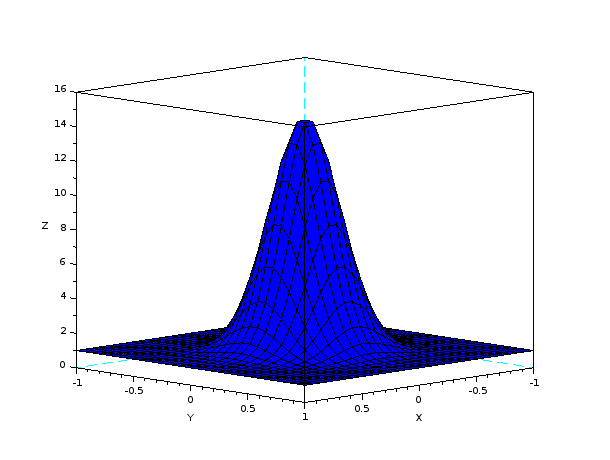
\includegraphics[scale=0.5]{Images/gaussienne.png}
\caption{La gaussienne}
\label{gaussienne}
\end{center}
\end{figure}



On choisit ensuite la solution $\displaystyle u(x,y) = \frac{x^4 + y^4}{4}$, qui nous donne, en prenant son gradient, la map suivante :

\begin{equation}
\displaystyle \nabla u (x,y) = \begin{pmatrix}x^3\\y^3 \end{pmatrix} 
\end{equation}

Cette map (fig.~\ref{mapchoisie}) sépare la gaussienne dans les 4 quadrants du repère. Pour obtenir le résultat du
mapping, on calcule :


$$ \rho_Y(x) =  \det(D^2 u(x) \rho_X(\nabla u(x)), \; \forall x \in X $$



et nous obtenons le résultat
représenté sur la figure \ref{resultmappage}.

\begin{figure}
\begin{center}
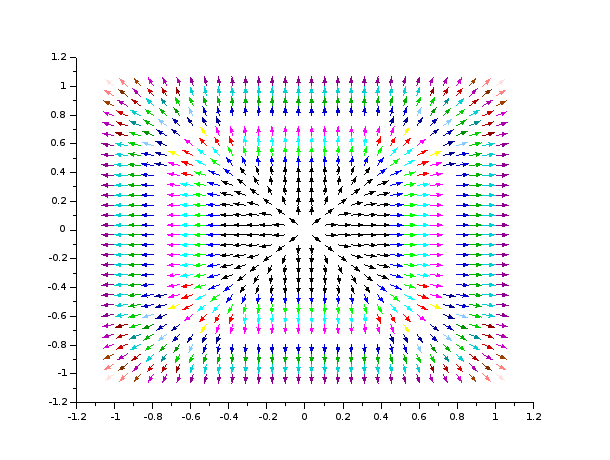
\includegraphics[scale=0.5]{Images/mapchoisie.png}
\caption{Map choisie}
\label{mapchoisie}
\end{center}
\end{figure}


\begin{figure}
\begin{center}
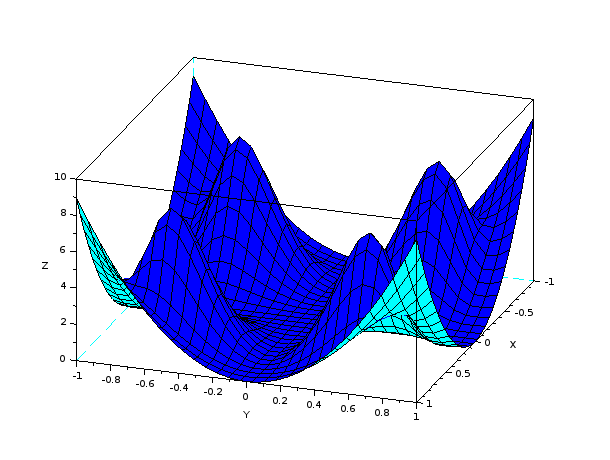
\includegraphics[scale=0.5]{Images/resmapchoisie.png}
\caption{Résultat du mappage}
\label{resultmappage}
\end{center}
\end{figure}


\subsection{Méthode de résolution}

La méthode de résolution que nous avons implémentée est celle qui est proposée dans \cite{benamou2014numerical}.

Il s'agit d'utiliser simultanément 3 schémas aux différences finies. Les deux premiers servant à résoudre l'équation
de Monge-Ampère, le troisième servant à calculer la condition au bord. \\


Les opérateurs aux différences finies utilisées sont :

\begin{align*}
[D_{x_1 x_1 }u]_{i,j} &= \frac{1}{dx^2} (u_{i+1,j} + u_{i-1,j}  - 2u_{i,j}) \\
[D_{x_2 x_2 }u]_{i,j} &= \frac{1}{dx^2} (u_{i,j+1} + u_{i,j-1}  - 2u_{i,j}) \\
[D_{x_1 x_2 }u]_{i,j} &= \frac{1}{4dx^2} (u_{i+1,j+1} + u_{i-1,j-1} - u_{i-1,j+1} -  u_{i+1,j-1}) \\
[D_{x_1 }u]_{i,j} &= \frac{1}{2dx} (u_{i+1,j} - u_{i-1,j} )\\
[D_{x_2 }u]_{i,j} &= \frac{1}{2dx} (u_{i,j+1} - u_{i,j-1} ) \\
\end{align*}

On utilise également des différences finies selon les directions $v = (\frac{1}{\sqrt{2}},\frac{1}{\sqrt{2}})$
et $v^{\perp} = (\frac{1}{\sqrt{2}},-\frac{1}{\sqrt{2}})$ :

\begin{align*}
[D_{v v }u]_{i,j} &= \frac{1}{2dx^2} (u_{i+1,j+1} + u_{i-1,j-1}  - 2u_{i,j}) \\
[D_{v^{\perp} v^{\perp} }u]_{i,j} &= \frac{1}{2dx^2} (u_{i+1,j-1} + u_{i-1,j+1}  - 2u_{i,j}) \\
[D_{v}u]_{i,j} &= \frac{1}{2\sqrt{2}dx} (u_{i+1,j+1} - u_{i-1,j-1} )\\
[D_{v^{\perp} }u]_{i,j} &= \frac{1}{2\sqrt{2}dx} (u_{i+1,j-1} - u_{i-1,j+1} ) \\
\end{align*}




Les deux schémas pour l'équation de Monge-Ampère sont un schéma monotone, noté MAM, et un schéma plus précis, noté MAA : 

\begin{equation}
MAA = D_{x_1 x_1}uD_{x_2 x_2}u - (D_{x_1 x_2}u)^2 - \rho_X / \rho_Y (D_{x_1}u,D_{x_2}u) - u_0
\end{equation}

\begin{align*}
MA1 &= max\lbrace  D_{x_1 x_1}, \delta \rbrace max\lbrace  D_{x_2 x_2}, \delta \rbrace -
min\lbrace  D_{x_1 x_1}, \delta \rbrace - min\lbrace  D_{x_2 x_2}, \delta \rbrace - \rho_X / \rho_Y (D_{x_1}u,D_{x_2}u) - u_0 \\
MA2 &= max\lbrace  D_{v v}, \delta \rbrace max\lbrace  D_{v^{\perp} v^{\perp}}, \delta \rbrace -
min\lbrace  D_{v v}, \delta \rbrace - min\lbrace  D_{v^{\perp} v^{\perp} }, \delta \rbrace - \rho_X / \rho_Y (D_{v}u,D_{v^{\perp}}u) - u_0 \\
MAM &= min \lbrace MA1, MA2 \rbrace
\end{align*}

Un filtrage permet, une fois les deux schémas calculés, de les mélanger correctement.

\subsection{Implémentation Scilab}
Nous avons
commencé par implémenter le schéma précis
présenté plus haut.

Par soucis de simplicité et de temps, mais aussi parce qu'elle sera plus facile à implémenter sous OpenCL par la
suite,  nous avons utilisé une itération explicite (Euler) au lieu de la méthode de Newton qui était conseillée dans \cite{benamou2014numerical}. Cette méthode est sujette à une condition CFL très restreinte
qui nous force à utiliser un pas de descente très petit. De ce fait, la convergence se fait très lentement.

L'itération s'écrit :

\begin{equation}
\displaystyle \frac{du}{dt} = \det(D^2 u) - \frac{\rho_X}{\rho_Y(\nabla u)}, \; x \in X
\end{equation}


Nous avons ensuite implémenté la condition au bord. Celle-ci est compliquée à implémenter, en particulier
il est difficile de réaliser les calculs efficacement. Il est absolument nécessaire de précalculer la plupart
des opérations  pour n'avoir à les faire qu'une seule fois au début du programme. Pour les détails, voir \cite{benamou2014numerical}.  \\

Enfin, nous avons implémenté le schéma monotone. Celui-ci est compliqué, il subsiste des bugs que nous n'avons pas
pu corriger par manque de temps, en particulier
sur l'intéraction avec le bord. Il est cependant fonctionnel à l'intérieur du domaine. Je suspecte l'existence de
fautes de frappe dans \cite{benamou2014numerical}, notamment dans les différences finies et le détail des schémas.

\subsection{Résultats}

En reprenant l'exemple vu plus haut et en calculant cette fois numériquement u, on voit que notre implémentation
converge bien vers la solution attendue (figure \ref{iterations}).

\begin{figure}
\begin{center}
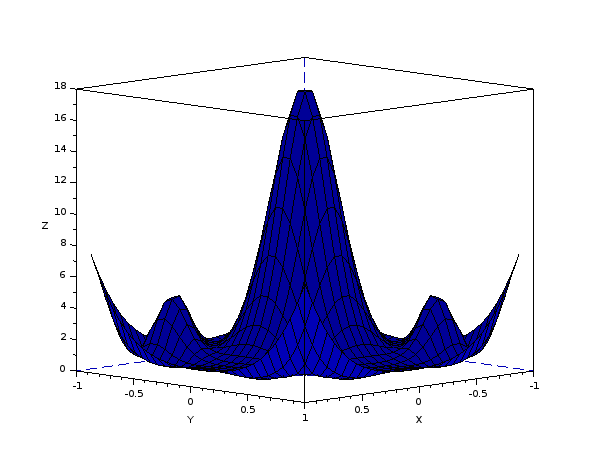
\includegraphics[scale=0.35]{Images/iter.png}
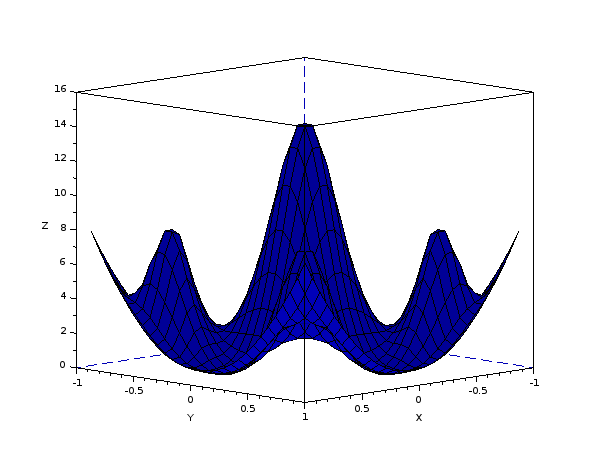
\includegraphics[scale=0.35]{Images/iter2.png}
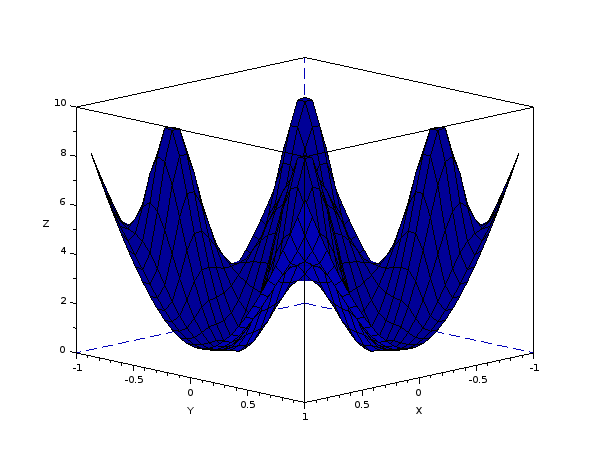
\includegraphics[scale=0.35]{Images/iter3.png}
\caption{Iterations 140, 200, et 700}
\label{iterations}
\end{center}
\end{figure}


Nous avons ensuite essayé de mapper la densité uniforme sur une gaussienne centrée en zéro. L'implémentation converge,
lentement mais sûrement, vers la solution attendue (figure \ref{iterationsg}).


\begin{figure}
\begin{center}
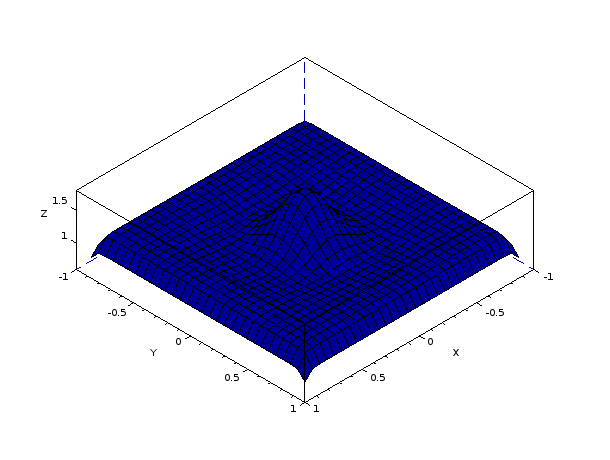
\includegraphics[scale=0.35]{Images/itergaussienne0.png}
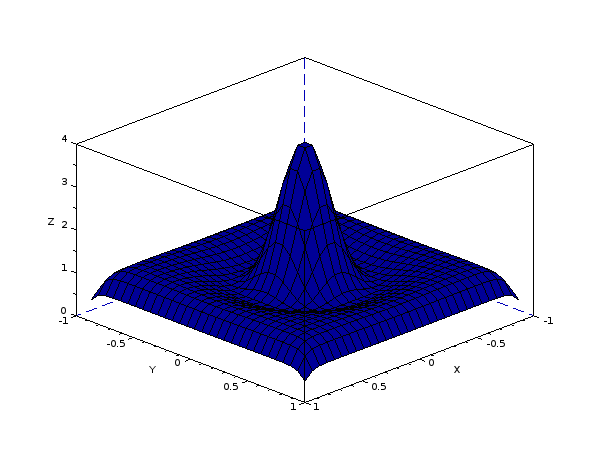
\includegraphics[scale=0.35]{Images/itergaussienne1.png}
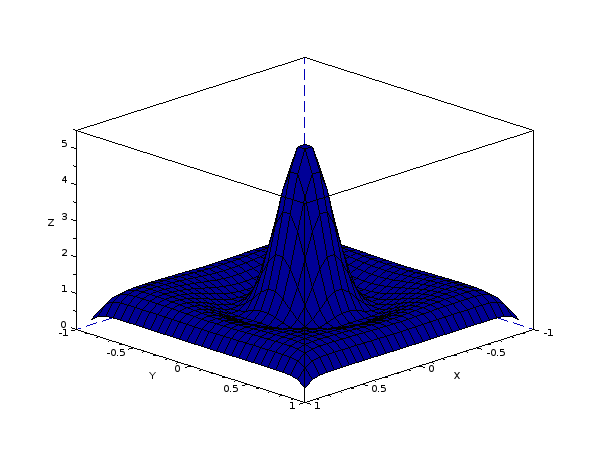
\includegraphics[scale=0.35]{Images/itergaussienne2.png}
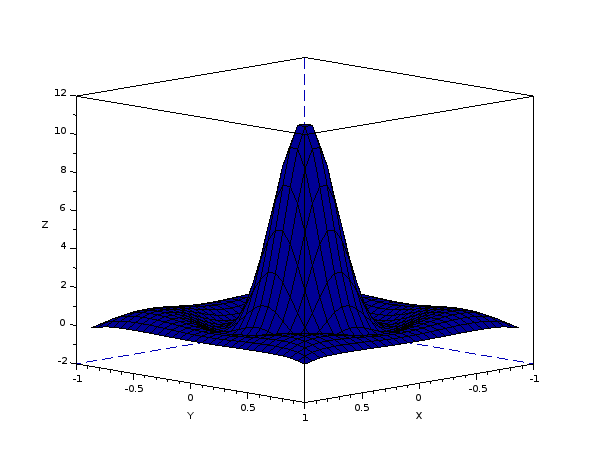
\includegraphics[scale=0.35]{Images/itergaussienne3.png}
\caption{Iterations 5, 50, 100 et 200 pour le mappage d'une gaussienne sur la densité uniforme}
\label{iterationsg}
\end{center}
\end{figure}


Idem, en essayant de déplacer une gaussienne sur une autre située en un autre endroit (figure \ref{iterationsg2}).



\begin{figure}
\begin{center}
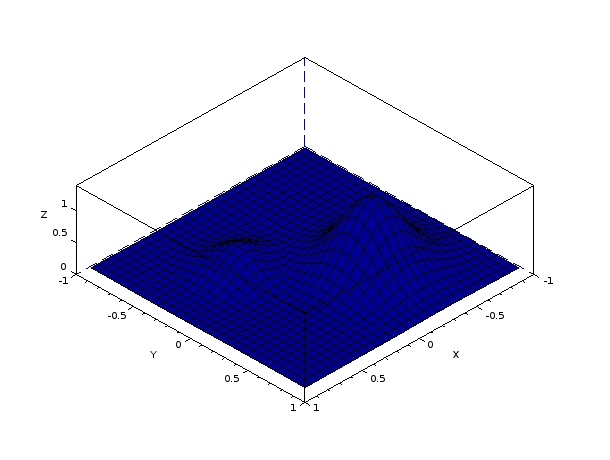
\includegraphics[scale=0.35]{Images/deplace1.png}
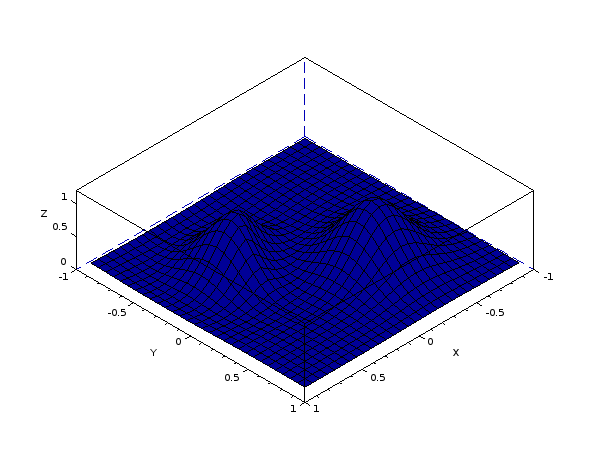
\includegraphics[scale=0.35]{Images/deplace2.png}
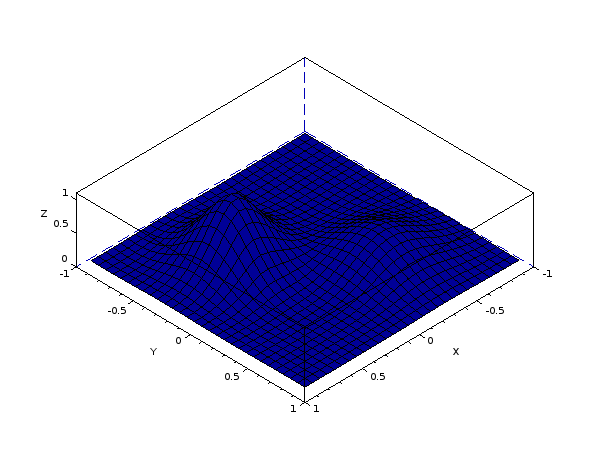
\includegraphics[scale=0.35]{Images/deplace3.png}
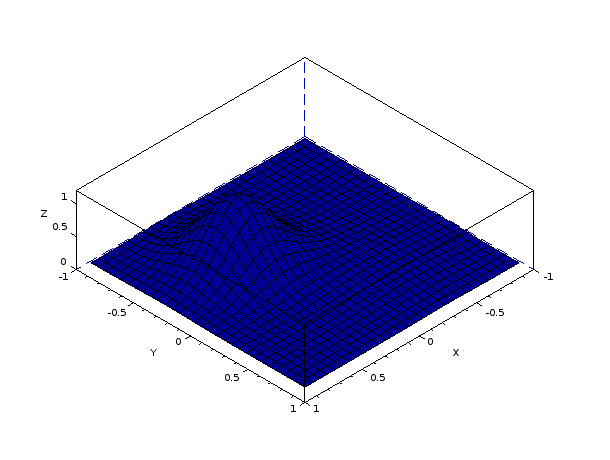
\includegraphics[scale=0.35]{Images/deplace4.png}
\caption{Iterations pour le mappage d'une gaussienne sur une autre}
\label{iterationsg2}
\end{center}
\end{figure}

Nous avons ensuite essayé un cas plus complexe avec des densités non continues. Il s'agit de déplacer un disque.
L'algorithme converge vers une solution qui est proche de celle qui doit être trouvée.


\begin{figure}
\begin{center}
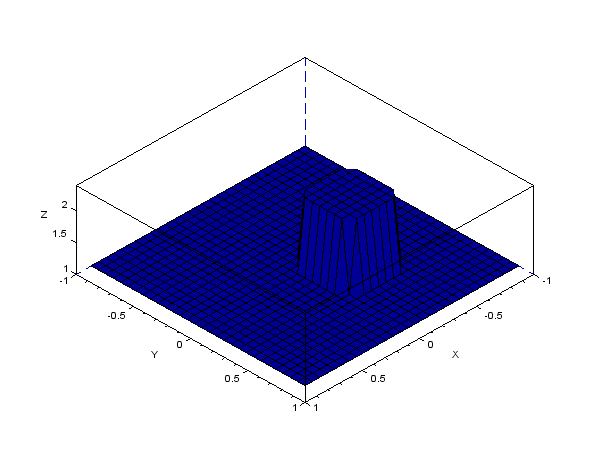
\includegraphics[scale=0.35]{Images/cercle1.png}
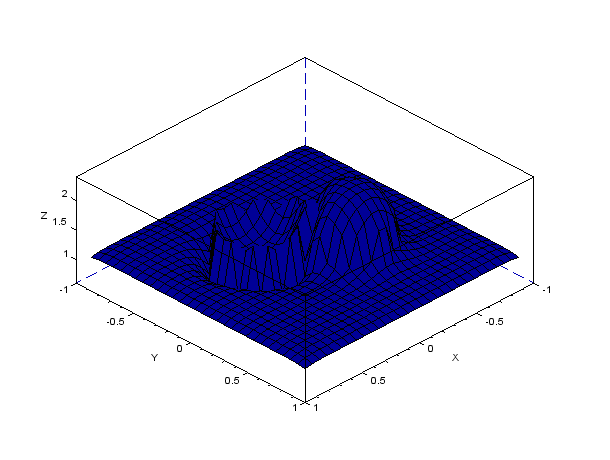
\includegraphics[scale=0.35]{Images/cercle2.png}
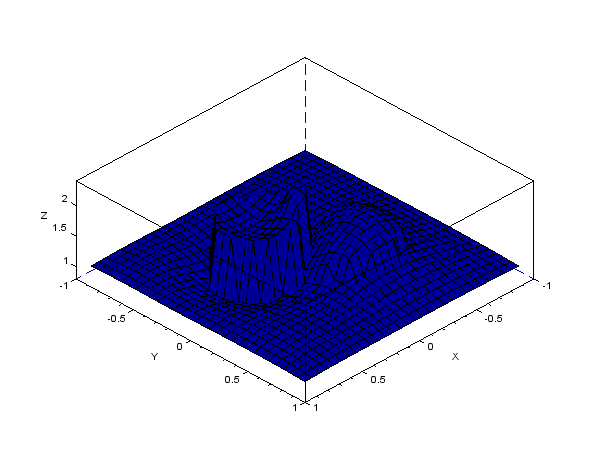
\includegraphics[scale=0.35]{Images/cercle3.png}
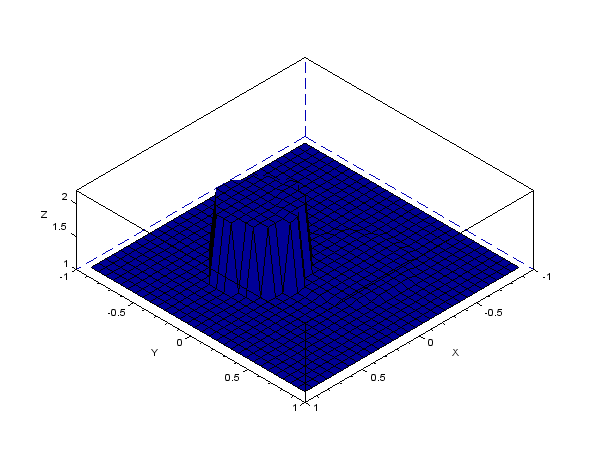
\includegraphics[scale=0.35]{Images/cercle4.png}
\caption{Iterations 1, 15, 80, et 500 pour le déplacement d'un disque}
\label{iterationsg2}
\end{center}
\end{figure}





\subsection{Implémentation OpenCL}

\subsubsection{Qu'est-ce qu'OpenCL ?}

OpenCL (pour \emph{Open Compute Language}) et un langage proche du C permettant de faire facilement du calcul parallèle pour différentes plate-formes d'execution\cite{stone2010opencl}. En particulier, les processeurs classiques (CPU) et les processeurs graphiques (GPU). Il est également possible d'utiliser d'autres types de puces, notamment les accélérateurs 
Xeon Phi d'Intel.

Il est similaire à CUDA dans son fonctionnement, mais je ne pouvais pas utiliser ce dernier car il ne fonctionne
que sur les cartes graphiques Nvidia. \\

\subsubsection{Qu'est-ce qu'un GPU ?}

Un GPU, ou \emph{Graphics Processing Unit}, est une puce étant à l'origine dédiée à l'affichage 2D et 3D. Elle est
constituée de centaines, voire milliers de petits processeurs, qui vont tous exécuter la même tâche au même moment.
Récemment, les GPU ont commencé à être utilisés pour du calcul scientifique, car leur architecture permet une 
haute parallélisation des tâches, ce qui est très pratique pour de la simulation, du calcul matriciel, etc.

\subsubsection{Travail réalisé}

Les différences finies dont nous avons besoin peuvent être calculées indépendamment pour chaque point de la grille.
Notre problème peut donc très fortement bénéficier de la parallélisation.


Seul le schéma MAA a été implémenté en OpenCL, et exécuté sur le circuit graphique d'une puce Intel Ivy Bridge.
Les gains en vitesse obtenus en passant sur GPU sont très importants, surtout en comparaison avec la vitesse
que nous avions sur Scilab.

Le GPU nous permet également d'obtenir plus de précision, car il est possible d'augmenter significativement le nombre
de points
de la grille sur laquelle nous travaillons. En effet, la vitesse avec une grille de 30 par 30 sous Scilab est environ
la même qu'avec une grille de 5000 par 5000 sur GPU (environ 2 itérations par seconde) !

\subsubsection{Détails d'implémentation}

Deux programmes ont été écrits à l'aide du SDK OpenCL d'Intel et de la documentation d'OpenCL \cite{khronos2009khronos}:

\begin{itemize}
\item Le premier s'exécute sur le processeur hôte (CPU). Il se charge d'initialiser et de lancer les calculs. En
particulier, il alloue des \emph{buffers} sur le GPU pour contenir les données après les avoir initialisées. Il 
récupère les résultats une fois que le GPU a terminé les calculs.

\item Le deuxième, appelé \emph{kernel}, est exécuté sur chaque processeur de flux du GPU. C'est celui qui va 
calculer les différences finies et mettre à jour la solution. Dans notre implémentation, le kernel réalise la
mise à jour de la solution $u$ en un seul point de la grille. Les différents points de la grille sont divisés en
tâches, qui vont être réparties entre les différents processeurs de flux. \\

\end{itemize}


Dans une implémentation itérative classique, la mise à jour de la solution se fait à l'aide d'une boucle \emph{for}. 
Pour passer à OpenCL, il faut prendre l'intérieur de la boucle, pour le mettre dans le \emph{kernel}. \\

Le programme hôte est composé de plusieurs étapes, qui doivent être réalisées avant le calcul. Elles entraînent
un certain temps de mise en place, appelé \emph{overhead}. Il faut : allouer les buffers sur l'hôte, les initialiser, allouer les buffers sur le GPU, copier les buffers de l'hôte au GPU, compiler le \emph{kernel} pour l'achitecture spécifique de notre GPU, positionner les arguments du \emph{kernel}, et enfin le lancer. Ces opérations sont
chacune une source potentielle d'erreurs (manque de mémoire sur l'hôte, manque de mémoire sur le GPU, erreur de compilation du kernel, absence de GPU,...), il est donc important de vérifier la valeur de retour de chacune des fonctions afin
d'être au courant de l'emplacement des erreurs que l'on rencontre, pour mieux déboguer le programme.

\subsubsection{Résultats}

Nous avons tout d'abord essayé de retrouver les résultats de la partie précédente.
Pour le déplacement de la gaussienne, l'application calculée est la même que celle calculée par Scilab (cf fig. \ref{cl}). Celle-ci a été calculée en 0,15s par le GPU, contre 1min10s sous Scilab.


\begin{figure}
\begin{center}
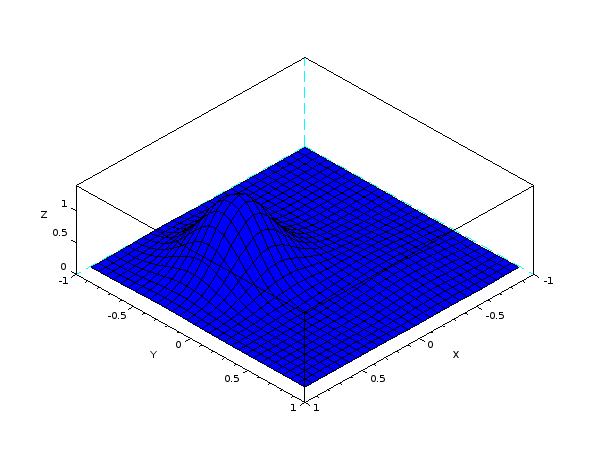
\includegraphics[scale=0.35]{Images/clrhoY30.png}
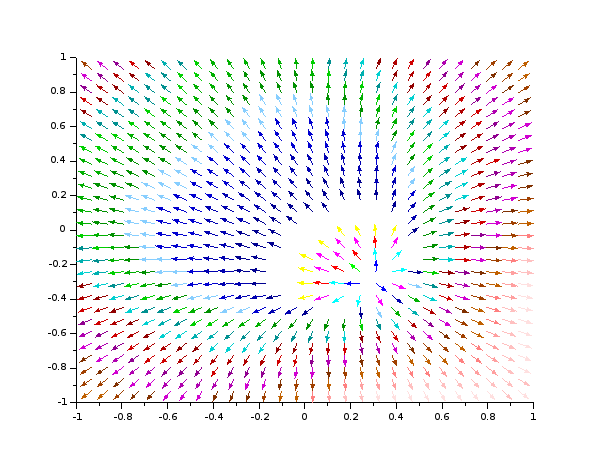
\includegraphics[scale=0.35]{Images/mapcl30.png}
\caption{Résultat obtenu après 1000 itérations sous OpenCL, avec une grille de 30x30}
\label{cl}
\end{center}
\end{figure}

Ensuite, nous avons décidé de calculer ce même déplacement, mais sur une grille de $256\times 256$ (cf fig \ref{cl2}). Dans ce cas, la condition CFL est encore plus restrictive, et nous avons besoin d'un nombre très important
d'itérations. Le GPU a calculé 200000 itérations en 45s. Une seule itération sous Scilab a pris 24s, il aurait donc 
fallu un peu moins de 8 semaines pour terminer le calcul sous Scilab.


\begin{figure}
\begin{center}
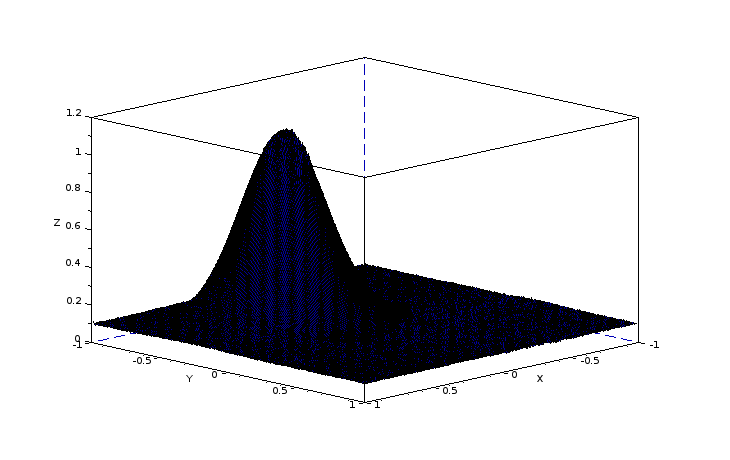
\includegraphics[scale=0.35]{Images/clres256.png}
\caption{Résultat obtenu après 200000 itérations sous OpenCL, avec une grille de 256x256}
\label{cl2}
\end{center}
\end{figure}


\newpage

\section{Conclusion}


\subsection{Résumé}

Durant cette Introduction à la Recherche en Laboratoire, nous avons étudié une nouvelle notion de solution d'Équation aux Dérivées Partielles. Nous avons implémenté un schéma numérique résolvant l'équation de
Monge-Ampère, tiré d'un article de recherche, et nous l'avons ensuite ré-implémenté en OpenCL pour être exécuté sur 
processeur graphique. \\

Nous avons obtenu des gains très importants avec le passage sur GPU, en particulier, le temps d'exécution de notre
méthode d'itération (itération explicite) sur GPU est maintenant du même ordre de grandeur que le temps 
d'exécution de la méthode de Newton implémentée dans l'article duquel nous avons tiré notre schéma \cite{benamou2014numerical}.

\subsection{Perspectives}

Les perspectives d'amélioration sont très claires. Puisqu'il subsiste des erreurs dans le schéma $MAM$, il faut
les trouver et les résoudre, ce que je n'ai malheureusement pas eu le temps de faire. Une fois le problème 
corrigé, il sera aussi possible d'implémenter ce schéma sous OpenCL. \\

Il est également possible de paralléliser
le schéma numérique utilisé pour résoudre l'équation d'Hamilton-Jacobi au bord du domaine et de le porter sous OpenCL. \\

La méthode de Newton pourrait également être implémentée. Cela n'a pas été fait ici car elle est plutôt 
complexe dans le cas de ce schéma numérique, et aurait donc été difficile à implémenter dans le temps imparti,
autant en Scilab qu'en OpenCL.

\subsection{Bilan de l'IRL}

Ce travail de recherche a été pour moi très enrichissant. J'ai pu approfondir et mettre en pratique des 
connaissances étudiées en MMIS, ce qui m'a permis de prendre un peu de recul par rapport à ce que nous
avons étudié au premier semestre. \\

Ayant fait un stage en laboratoire de recherche l'été dernier, je ne peux pas dire que je ai découvert l'ambiance
d'un laboratoire uniquement grâce à l'IRL. J'ai cependant eu l'occasion de mieux comprendre les méthodes de 
recherche, en particulier parce que mon sujet n'était pas intégralement défini lorsque l'IRL a commencé. 
J'ai en effet eu l'opportunité de choisir moi-même sur quel problème j'allais travailler après avoir compris
la notion de solution de viscosité. \\

J'ai pu, pendant ce semestre, assister à des séminaires de recherche au sein du Laboratoire Jean Kuntzmann, ce qui 
m'a permis de découvrir de nouvelles méthodes et de nouvelles applications des Équations aux Dérivées Partielles.
Ceci a nettement renforcée l'idée que j'ai de vouloir continuer dans la voie de la simulation et de l'optimisation.


\newpage
\bibliographystyle{ieeetr}
\bibliography{biblioIRL}


\newpage
\section{Annexe A : Code Scilab}

\lstinputlisting[language = Scilab, frame = single, basicstyle=\footnotesize\ttfamily,breaklines=true]{../progs/thing.sce}


\section{Annexe B : Code OpenCL}
\lstinputlisting[language = C, frame = single, basicstyle=\footnotesize\ttfamily,breaklines=true]{../progs/ClImplem/MongeAmpereKernels.cl}
\lstinputlisting[language = C, frame = single, basicstyle=\footnotesize\ttfamily,breaklines=true]{../progs/ClImplem/MongeAmpere.cpp}
%\end{spacing}
\end{document}
